% Chapter 3

\chapter{GNSS实时滤波精密轨道确定的研究与实现}

\section{引言}

不论是提供事后或是实时的导航卫星轨道的位置服务,目前主流的GNSS精密轨道处理的方式仍是基于事后批处理的解算模型,其算法模型和处理流程随着多年来研究已经逐步趋于完善。相对的,基于实时观测数据,采用实时滤波解算方式进行轨道确定的处理模式在近几年仍在不断的研究和探索中。在事后批处理过程中,由于包含了所有观测数据信息,因此可以对观测数据进行统一的预处理,同时在解算过程中进行反复迭代计算和整体质量控制,以达到最优的数据处理效果。而实时滤波处理流程中往往需要通过处理实时观测数据流,实时给出当前已有观测数据信息下的最优轨道位置信息。因此实时滤波精密轨道确定在不论是在观测数据的预处理、参数估计方法、质量控制方法以及整体算法流程都与事后解算模式大不相同。如果直接应用事后解算模式的经验与方法,将难以取得理想的解算效果。

本章从实时滤波精密轨道确定的算法流程出发,分别对处理过程中的关键环节:参数估计方法、实时质量控制方法和实时模糊度固定方法,进行了相应的推导和实现,并通过实验对比分析验证了算法的正确性和有效性。最后,本文在目前已有的数据处理软件平台上GREAT(GNSS+ Research,
Application and Teaching)的基础上,开发实现了具有GNSS实时滤波精密轨道确定的功能,并给出了该功能的整体结构组成及其算法处理流程。

\section{基于平方根信息滤波的参数估计原理}

在第二章的参数估计部分,我们介绍了常用的最小二乘算法和卡尔曼滤波估计算法。其中卡尔曼滤波估计算法更适合实时数据的处理,相对于最小二乘批处理需要存储所有的观测值信息,滤波估计算法无需存储历史时刻的观测数据信息,而是以待估参数的协方差矩阵信息进行存储。同时滤波算法在处理具有先验运动模型的最优估计问题也更为直观。但由于计算机中计算过程截断误差的存在,导致存在滤波因数值误差而发散的情况存在,因此引入了平方根滤波相关的算法(Dyer,1969),其核心原理通过采用原有滤波算法一半字节长度进行相关数据信息的存储,大大减少了数值计算误差,从而抑制了滤波发散的情况,具有更高的数值稳定性。这里,我们选用了实时滤波轨道处理中常用的平方根信息滤波(Square Root Information Filter,SRIF)作为参数估计的方法。由于广义最小二乘算法在测绘领域更为常用,因此本文从广义最小二乘算法角度出发,推导和梳理了SRIF算法过程。

\subsection{量测更新算法}

对于已经构建好线性化后的观测函数模型以及确定了待估参数的问题中,最小二乘算法所求解的核心问题为:在包含有多余观测量的情况下,求解出一组最优的待估参数,使得所有观测方程的残差平方和最小,即满足式\eqref{eq:define_LSQ}。
    \begin{equation}
        \begin{aligned}
		& \nu = A_{m\times{n}}x_{n\times{1}}-b_{m\times{1}},P \\
		& \nu^{T}P\nu=min
        \end{aligned}
        \label{eq:define_LSQ}
    \end{equation}
式中,\(x\)为待估计的参数向量,\(A\)为观测函数模型化对在参数初始值上的线性化后的系数矩阵,\(b\)为观测值与使用参数初值计算的观测函数初值之差得到的先验残差向量。\(m,n\)分别为观测方程的数量与待估参数的维度。\(P\)为观测方程的权矩阵,这里假定其为正定对称阵。在此基础上,除考虑观测信息外,还需要考虑到待估计参数具有先验信息\(W\)。这里广义最小二乘算法的常见做法是构建基于先验的虚拟观测方程,和其他观测方程一同求解,即式\eqref{eq:define_LSQ}可以被扩展成式\eqref{eq:LSQ_more}。
    \begin{equation}
        \begin{aligned}
		& \nu =A_{new}x-b_{new},P_{new} \\ 
		& A_{new} = 
		\begin{bmatrix}
			E \\
			A 
		\end{bmatrix},
		b_{new} = 
		\begin{bmatrix}
			\bar{x}\\
			b
		\end{bmatrix},
		P_{new}=
		\begin{bmatrix}
			W & 0 \\
			0 & P
		\end{bmatrix}\\
        \end{aligned}
        \label{eq:LSQ_more}
    \end{equation}
式中,\(E\)为单位阵,\(\bar{x}\)为待估参数的先验值。

这里为了求解式\eqref{eq:LSQ_more},可以等价求解其对应的正规方程(normal equations),即\(A^{T}PAx=A^{T}Pb\)。当观测系统存在病态观测的时候,也就是系数矩阵\(A\)的条件数较大的时候,容易导致所求解的参数数值误差较大。为了避免这种情况,可以使用QR分解的方式进行求解。在使用QR分解算法之前,需要对上述广义最小二乘问题进行单位权规整化。对于前述的观测方程权矩阵和先验信息的权矩阵作三角化分解有,\(P=\varepsilon_{k}^{T}\varepsilon_{k},W=R_{k}^TR_{k}\),这里我们用下标\(k\)表明权矩阵所在时刻,因此,上述最小二乘问题可被等价转换为下面的表达:
\begin{equation}
	\begin{aligned}
	& min(\nu^{T}P\nu) =min \Vert Hx-l \Vert_{2} \\
	& H = 
	\begin{bmatrix}
		\varepsilon_{k}\\
		R_{k}A 
	\end{bmatrix}x ,
	l = 
	\begin{bmatrix}
		\varepsilon_{k}\bar{x} \\
		R_{k}b 
	\end{bmatrix}
	\end{aligned}
	\label{eq:LSQ_single}	
\end{equation}
式中,\(H,l\)分别表示规整化后的系数矩阵与先验残差向量。对系数矩阵进行QR分解有:
\begin{equation}
	\begin{aligned}
		& H_{m \times n}=
		\begin{bmatrix}
		\varepsilon_{k,m \times n}\\
		R_{k}A_{(m-n) \times n }
		\end{bmatrix} = 
		Q_{m \times m}
		\begin{bmatrix}
		\varepsilon_{k+1/k,m \times n}\\
		0_{(m-n) \times n}
		\end{bmatrix} \\ 
		& QQ^{T}=E
	\end{aligned}
	\label{eq:QR_factor}
\end{equation}
式中,\(Q\)为分解得到的正交矩阵。对式\eqref{eq:LSQ_single} 左右两边同乘以\(Q^{T}\),则可以得到相应的等价表达:
\begin{equation}
	\begin{aligned}
		min \Vert Hx-l \Vert_{2} & = min(\Vert
		\begin{bmatrix}
			\varepsilon_{k+1/k} \\
			0
		\end{bmatrix} x-Q^{T}
		\begin{bmatrix}
			\varepsilon_{k}\bar{x} \\
			R_{k}b 
		\end{bmatrix}
		 \Vert _{2})\\
		& = min(\Vert \varepsilon_{k+1/k}x - z \Vert_{2} +
			\Vert e \Vert_{2}
		)\\		
		& = min(\Vert \varepsilon_{k+1/k}x - z \Vert_{2}) \\
		z & = Q^{T}\varepsilon_{k}\bar{x},
		e= Q^{T}R_{k}b
	\end{aligned} 
\end{equation}
式中,\(e\)为正规化后的验后观测残差向量。此时待估参数可以直接用由\(\varepsilon_{k+1/k}^{-1}x=z\)直接求解得到,该方程在SRIF中也也被称为信息方程。到可以发现此表达式与k时刻的规整化的先验信息虚拟观测方程类似,此时\(\varepsilon_{k+1/k}^{T}\varepsilon_{k+1/k}\)即为求解后参数\(x\)的信息权矩阵,这里我们已经完成了SIRF量测更新的推导。在SRIF中,\(\varepsilon\)为待估参数的信息矩阵,因为其为原有的先验信息权矩阵三角化后的结果,在数值计算上具有更好的稳定性,其量测更新的核心原理即为式\eqref{eq:QR_factor},其中分解得到\(\varepsilon_{k+1/k}\)即可直接作为量测更新后参数的信息矩阵。

\subsection{时间更新算法}

导航卫星精密轨道确定问题中包含着大量的随时间变化的动态参数,如轨道参数、钟差参数、对流层参数和模糊度参数等。
如何在SRIF算法中随时间动态更新调整这些参数,也是实时滤波轨道处理中的一个关键步骤。
尽管这些动态参数各自具有不同的特性,但考虑它们一般化的时间更新过程,都包含了参数增加、参数状态更新、参数消除这三个部分。
接下来依次对这三个部分的具体算法流程进行相应的介绍

考虑j时刻的信息方程为\(\varepsilon_{j}x=z_{j}\)。其中,我们将参数\(x\)中分为两个类别\(x^{T}=[x_{r,j},x_{c}]\),其中\(x_{r,j}\)表示过了j时刻后需要消除的参数,\(x_{c}\)表示过了j时刻还需要保留的参数。假定\(\varepsilon_{j}\)的信息矩阵为上三角阵(若不为上三角阵,可做一次QR分解后得到),此时信息方程可表示为如下形式:
\begin{equation}
	\begin{aligned}
		\begin{bmatrix}
			\varepsilon_{r,j} & \varepsilon_{rc,j} \\
			0 & \varepsilon_{c,j} \\
		\end{bmatrix}
		\begin{bmatrix}
			x_{r,j} \\
			x_{c,j}
		\end{bmatrix}
		 =
		\begin{bmatrix}
			z_{r,j} \\
			z_{c,j} \\	
		\end{bmatrix}
	\end{aligned}
\end{equation}
对于下个历元新增加的参数这里我们使用\(x_{n,j+1}\)进行表示。对于新增参数,考虑其具有的先验信息方程为\(\zeta_{j+1}x_{n,j+1}=z_{n,j+1}\)。因此根据类似式\eqref{eq:LSQ_more}的广义最小二乘原理,此时参数增加后的信息方程可以直接表示为如下形式:
\begin{equation}
	\begin{aligned}
		\begin{bmatrix}
		\varepsilon_{r,j} & \varepsilon_{rc,j} & 0 \\
		0 & \varepsilon_{c,j} & 0 \\
		0 & 0 & \zeta_{j+1} 
		\end{bmatrix}				
		\begin{bmatrix}
			x_{r,j}\\
			x_{c,j}\\
			x_{n,j+1}
		\end{bmatrix}	
		=
		\begin{bmatrix}
			z_{r,j}\\
			z_{c,j}\\
			z_{n,j+1}
		\end{bmatrix}
	\end{aligned}
	\label{eq:init_eq}
\end{equation}

考虑到\(x_{r,j}\)和\(x_{n,j+1}\)可以构建如下的状态变化方程:
\begin{equation}
	\begin{aligned}
	& x_{n,j+1} = \phi_{j+1/j}x_{r,j}+ \beta_{j+1/j},W_{\omega}   \\ 
	& W_{\omega}=R_{\omega}^{T}R_{\omega}
	\end{aligned}
	\label{eq:trans_eq}
\end{equation}
式中,\(\phi_{j+1/j}\)为线性化后的状态转移矩阵,\(W_{\omega}\)为状态转移方程的信息权矩阵,其三角化分解后的结果为\(R_{\omega}\),\(\beta_{j+1}\)为状态转移方程中的过程噪声,其大小一般与状态转移的时间间隔相关。
到这里可以发现,本质上完成参数的状态更新过程,即等价于将式\eqref{eq:trans_eq}当作观测方程,对式\eqref{eq:init_eq}的信息方程完成一次量测更新。因此对参数进行状态更新依然可以基于QR分解完成。这里我们仿照式\eqref{eq:LSQ_single}构造如下的最小二乘模型,并对系数矩阵进行QR分解,可以得到如式\eqref{eq:SRIF_timeupdate}的形式:
\begin{equation}
  \begin{aligned}
	 min(\Vert Hx-l \Vert_{2}) & = min(\Vert
	 \begin{bmatrix}
		\varepsilon_{r,j} & \varepsilon_{rc,j} & 0 \\
		0 & \varepsilon_{c,j} & 0 \\
		0 & 0 & \zeta_{j+1} \\
		-R_{\omega}\phi & 0 & R_{\omega}\\
	\end{bmatrix}
	\begin{bmatrix}
		x_{r,j}\\
		x_{c,j}\\
		x_{n,j+1}
	\end{bmatrix}
	-
	\begin{bmatrix}
		z_{r,j}\\
		z_{c,j}\\
		z_{n,j+1} \\
		R_{\omega}\beta_{j+1/j}
	\end{bmatrix}
	\Vert_{2} )\\
	& \Downarrow H = QR \\
	& = min(\Vert 
	\begin{bmatrix}
	\varepsilon_{r,j+1} & \varepsilon_{rc,j+1} & \varepsilon_{rn,j+1} \\
	0 & \varepsilon_{c,j+1} & \varepsilon_{cn,j+1} \\
	0 & 0 & \varepsilon_{n,j+1}\\
	0 & 0 & 0
	\end{bmatrix}
	\begin{bmatrix}
		x_{r,j}\\
		x_{c,j}\\
		x_{n,j+1}
	\end{bmatrix}
	-
	Q^{T}
	\begin{bmatrix}
		z_{r,j}\\
		z_{c,j}\\
		z_{n,j+1} \\
		R_{\omega}\beta_{j+1/j}
	\end{bmatrix}
	\Vert_{2})
  \end{aligned}	
  \label{eq:SRIF_timeupdate}
\end{equation}
式中,\(\varepsilon_{j+1}\)表示了j+1时刻下的信息方程的信息矩阵,\(Q\)为对系数矩阵进行QR分解得到的正交矩阵。这样便推导得到了参数状态过更新后的信息方程。
最后,可以发现由于信息矩阵为上三角矩阵,对于后续不再需要的\(x_{r,j}\)参数,可以很自然地将其对应的信息方程中的所在行删除,方程剩余的部分依然满足信息方程的结构。
同时,由于SRIF算法中的时间更新和量测更新是随时间不断地迭代进行,因此删除过时参数可以大大避免因为这些参数导致的无意义的计算资源的消耗。

至此,已经推导得到了基于QR分解实现时间更新基本原理。对于参数增加和消除,由于信息方程的上三角化的特殊结构,可以通过简单的矩阵变换得到。
对于参数状态更新的部分,其核心关键就在于构建式\eqref{eq:trans_eq}的状态转移方程以及式\eqref{eq:SRIF_timeupdate}的信息方程的时间更新。

\subsection{基于SRIF的实时滤波轨道处理流程}

(这里把轨道参数如何进行转移的问题进行相关阐述)
前面推导了平方根信息滤波的量测更新和时间更新的基本原理,图~\ref{fig:SRIF_flowchart}给出了出基于平方根信息滤波的实时滤波轨道的基本处理流程。
这里将实时滤波轨道中的时间更新分成了轨道参数与其他参数两个部分。其中,对于轨道参数的更新,我们通常需要通过数值积分获取前后历元的状态转移矩阵,从而构建相应的状态转移方程。但考虑到数值积分过程较为耗时,这里通常不需要在每个历元进行积分计算,而是使用之前的积分的计算结果进行一个近似地使用。对于轨道状态转移方程的权阵设定:
对于非轨道参数的更新,在无电离层模型中,主要需要考虑钟差参数、对流层参数、系统间偏差参数和模糊度参数的状态更新。
\begin{figure}
  \centering
  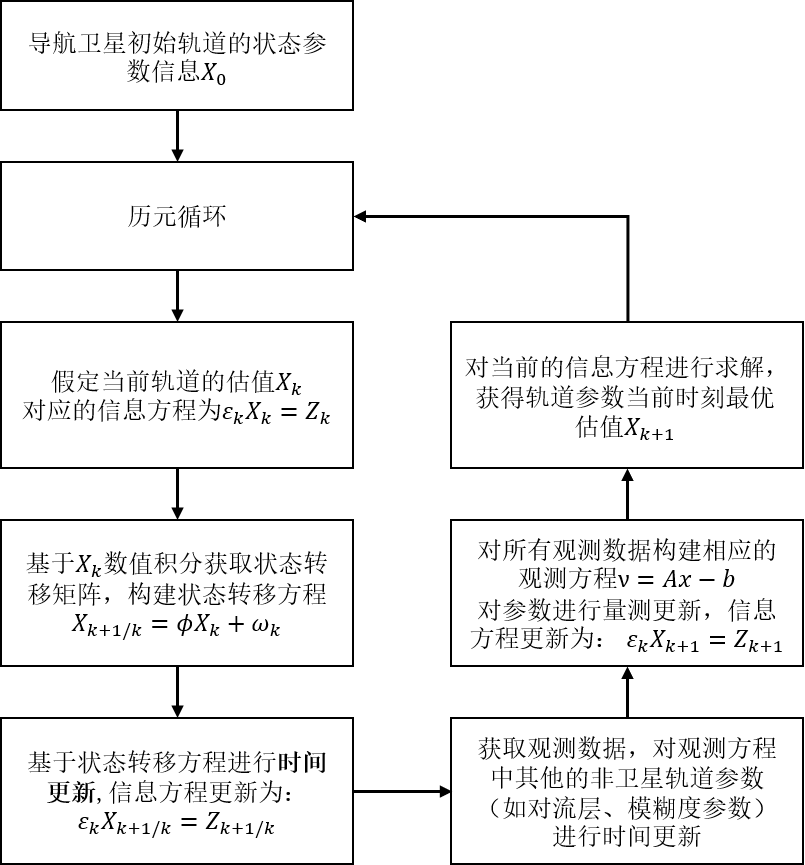
\includegraphics[width=0.6\textwidth]{SRIF_flowchart.png}
  \caption{基于SRIF的实时滤波轨道处理流程图}
  \label{fig:SRIF_flowchart}
\end{figure}


\section{GNSS数据的实时质量控制}

\begin{figure}
  \centering
  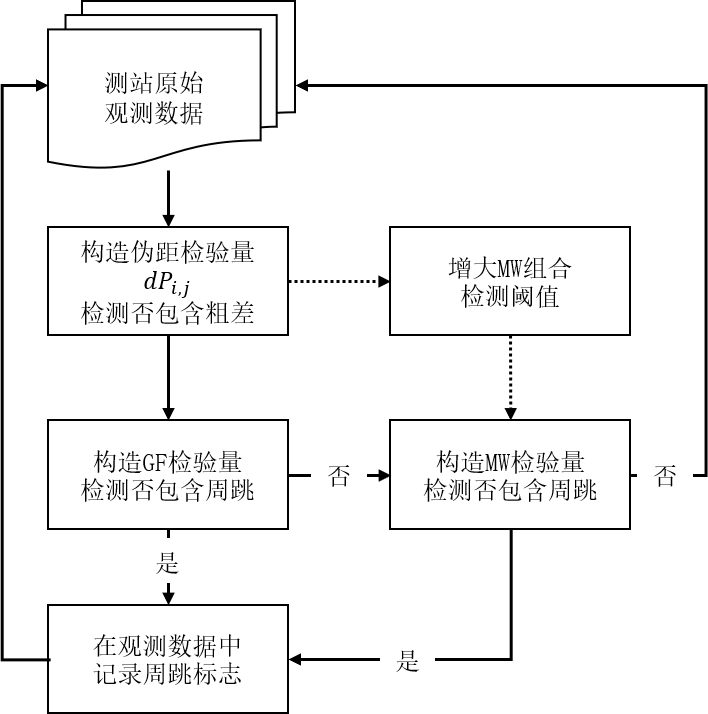
\includegraphics[width=0.6\textwidth]{preprocess.png}
  \caption{GNSS实时数据预处理算法流程图}
  \label{fig:tb_flowchart}
\end{figure}

\subsection{实时周跳探测算法}

\subsection{实时质量控制算法}


\subsection{实验结果和分析}

实验设计:

主要目的:选用经过多次迭代后的log\underline{\space}tb文件作为参考值,认为其中没有发生周跳。以此对比实时质量算法所起的作用。

分别使用该log\underline{\space}tb文件,以及实时周跳探测和质量控制的算法分别进行实时滤波轨道确定计算

实验方案: 110 个测站 10天的3d解(天数可以商榷) GPS单系统
方案1:使用log\underline{\space}tb进行计算(关掉了实时周跳探测以及实时质量控制,纯解算)

方案2:开启litetb(感觉需要使用300s的阈值,否则这样信息感觉比事后的tb解算多),其次是开启质量控制算法(即重置模糊度,这里需要测试不同max\_res\_norm阈值下的结果吗 这个感觉有点区别啊)

\section{实时双差模糊度固定方法}

\subsection{双差模糊度固定算法基本原理}

\subsection{实验结果和分析}

实验设计:

主要目的:
相较于浮点解,对比不同模糊度固定算法在实时轨道中所起的作用

实验方案:110个测站  10天的3d解,基于编辑残差后的log\_tb进行解算结果? GCE三系统的结果
同时对比不同的实验方案(紧约束的和松约束)

这里就直接说是基于残差log\_tb的结果算了,不过实际算的时候应该使用初始tb加上实时质量控制的算法

\section{实时滤波精密轨道处理软件结构}

画图画图再画图
